A validation sweep was run using six benchmarks. These
applications were run using UVM Smart model that approximates a Nvidia V100. The simulation parameters are shown in Table
\ref{tab:v100_params}. The overall kernel runtime was compared with the results
of running the six applications through nvprof on Nvidia Tesla V100. Figure \ref{fig:correlation}
shows the total number cycles that each application took on the simulation model
and on the native V100. Note that this is only cycles where a kernel was running
and does not include host execution time. The performance gap mainly comes from prefetching algorithms. The blue cross points represent the result of no prefetcher applied, the yellow represents random prefetched, the black represents the sequential locality prefetcher, and the cyan represents the tree-based neighbor prefetcher. It is very clear that the tree-based neighbor prefetcher has the best correlation, which seems very close to the tree-based hardware prefetcher implemented by NVIDIA CUDA driver.

   \begin{figure}[!htb]
      \centering
      \setlength{\abovecaptionskip}{6pt plus 1pt minus 1pt}
      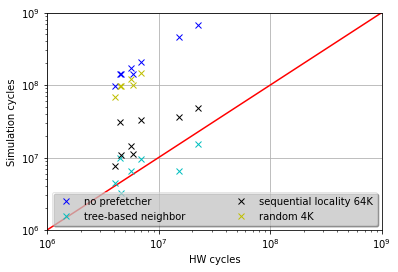
\includegraphics[width=.90\textwidth,keepaspectratio]{figures1/corre.elf}
      \captionsetup{width=.75\textwidth}
      \caption{Correlations between simulator and hardware.}
      \label{fig:correlation}
   \end{figure}


    \begin{table}[!htbp]
      \centering
      \setlength{\belowcaptionskip}{6pt plus 1pt minus 1pt}
      \captionsetup{width=.75\textwidth}
      \caption{CPU/V100 Model Parameters}
      \hspace{1cm}
         \begin{tabular}{|l|c|}
            \hline
            Clock                 & 1312MHz          \\ \hline
            SMs                   & 84               \\ \hline
            L2 Slices             & 32               \\ \hline
            L2 Capactiy           & 192KiB per slice \\ \hline
            HBM Capacity          & 16384MiB         \\ \hline
            HBM Stacks            & 4                \\ \hline
            Crossbar Frequency    & 1200MHz          \\ \hline
            Crossbar Input Ports  & 2                \\ \hline
            Crossbar Output Ports & 1                \\ \hline
         \end{tabular}
      \label{tab:v100_params}
   \end{table}